\documentclass[10pt]{beamer}
\setbeameroption{hide notes}
\usepackage{qcircuit}
\usepackage{braket}
\usepackage{tikz}
% \setbeameroption{show notes on second screen}
\usetheme[sectionpage=progressbar,numbering=counter,block=fill]{metropolis} % Use metropolis theme
\title{Qubits And Quantum Computers}
\date{}
\author{QuTe}
\logo{
\begin{tikzpicture}[overlay,remember picture]
  \coordinate (logo) at ([xshift=.0cm,yshift=.0cm]current page.south west);
  \node [anchor=south west] at (logo) {
\includegraphics[width=2cm]{img/erasmus_plus.jpg}};
\end{tikzpicture}
}
\titlegraphic{
\begin{tikzpicture}[overlay,remember picture]
  \coordinate (logo) at ([xshift=-.07cm,yshift=-.07cm]current page.south west);
  \node [anchor=south west] at (logo) {
\includegraphics[width=2cm]{img/erasmus_plus.jpg}};
\end{tikzpicture}
}

\begin{document}
\maketitle

\begin{frame}
  \section{Ready, set, go!}
  Grab your \emph{Qubits and Quantum Computers} notes and follow along!
\end{frame}

\begin{frame}
  \section{Bits and Qubits}
\end{frame}

\begin{frame}
  \frametitle{Bits}
  \begin{columns}
    \begin{column}{0.5\linewidth}
      \begin{itemize}
      \item<1-> Two state system
      \item<2-|alert@2> heads or tail
      \item<3-|alert@3> up or down 
      \item<4-|alert@4> charge or no charge
      \item<5-|alert@5> 0 or 1 
      \end{itemize}
    \end{column}
    \begin{column}{0.5\linewidth}
      \centering
      \includegraphics<2>[height=3cm]{img/euro-0.jpg}

      \includegraphics<2>[height=3cm]{img/euro-1.jpg}

      \includegraphics<3>[height=3cm]{img/keep-calm-its-just-a-bit-of-fun.png}
      \includegraphics<3>[height=3cm]{img/keep-calm-its-just-a-bit-of-fun_upside_down.png}

      \includegraphics<4>[height=3cm]{img/ssd.png}

      \onslide<5> \centering \Huge 0 1 
    \end{column}
  \end{columns}
\end{frame}

\begin{frame}
  \frametitle{Bits}
  \begin{block}{Exercise 1 p. 2 in the notes}
    How many possible combinations are possible with 4 bits? Same question but with 10 bits and with \emph{n} bits?
  \end{block}
\end{frame}

\begin{frame}
  \frametitle{A classical computer}
  \Large How many of the numbers are greater than 4?

  \centering 
  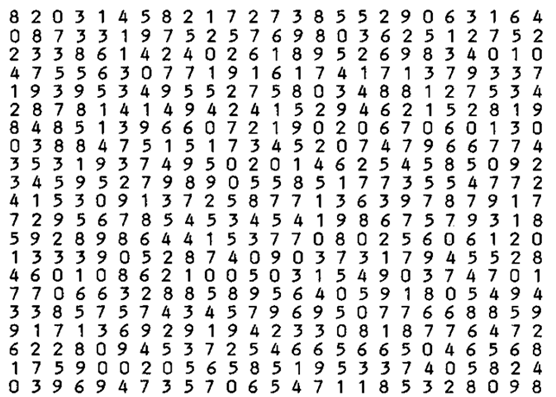
\includegraphics[scale=0.4]{img/random_numbers.png}

  \onslide<2> \normalsize Perfect for a classical computer: One thing at a time, very fast!
  
\end{frame}

\begin{frame}
  \frametitle{Unlock the bike}
  
  \begin{block}{Exercise 2 p. 2 in the notes}
    \begin{columns}
      \begin{column}{0.6\linewidth}
        The code cylinder on a bicycle lock is made up of 5 numbers between 0 and 9: How many possible combinations (i.e. how many codes) does the lock have?
      \end{column}
      \begin{column}{0.3\linewidth}

       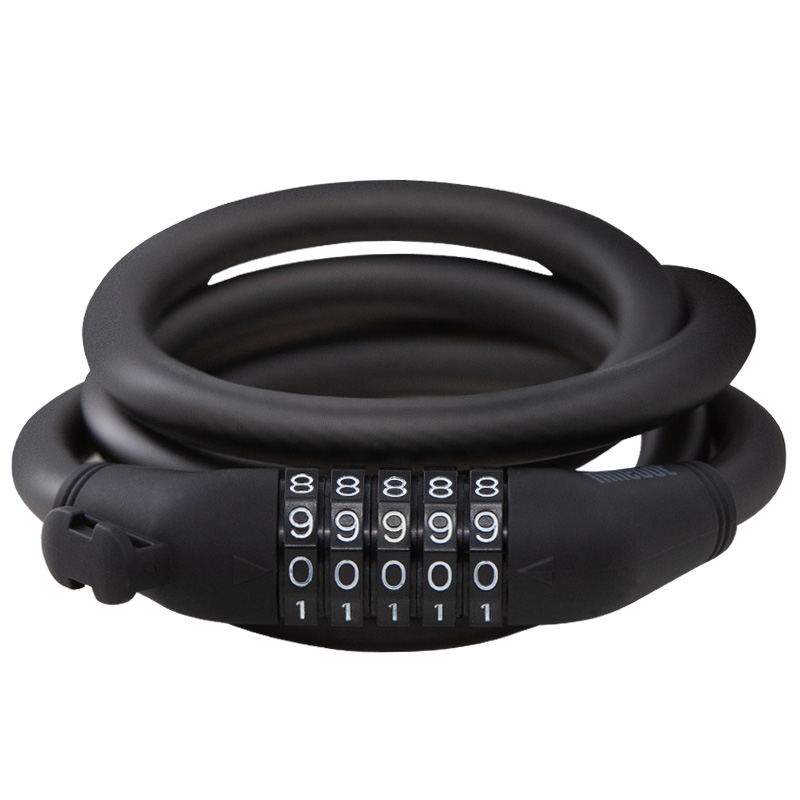
\includegraphics[width=\linewidth]{img/lock5.jpg} 

      \end{column}
    \end{columns}
  \end{block}
\end{frame}

\begin{frame}
  \frametitle{Complexity}
  \begin{columns}
    \begin{column}{0.5\linewidth}
      \begin{block}{Definition 1}
       Complexity of a calculation: the number of operations needed to find a solution to a given problem when the size of hte input is \emph{m}. 
      \end{block}
    \end{column}
    \begin{column}{0.5\linewidth}

      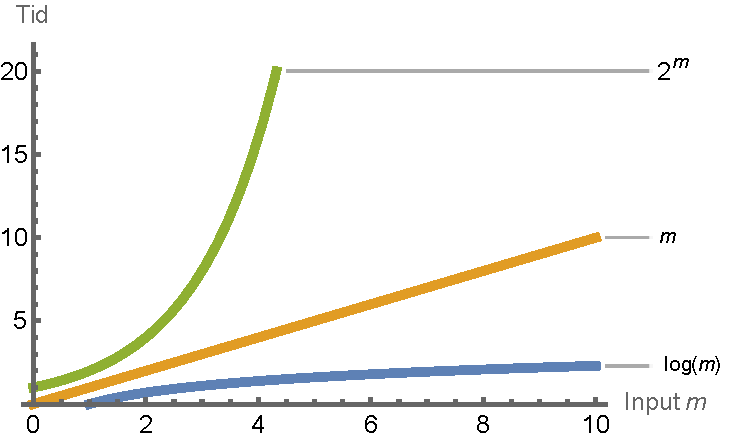
\includegraphics[width=\linewidth]{img/Complexity.pdf}
    \end{column}
  \end{columns}
  \onslide<2> \Large Often the problems increases \emph{exponentially}.
\end{frame}

\begin{frame}
  \frametitle{Exercises}
  \begin{block}{Exercise 3 p. 3 in the notes}
    \begin{columns}
    \begin{column}{0.6\linewidth}
    A classical supercomputer can perform $10^{17}$ operation each second. Vi use it to break a code lock like the one before, except with $m$ digits instead of 5. Assume that the classical supercomputer can check $10^{17}$ different combinations on the lock each second. How large can $m$ be if the classical supercomputer must be able to complete the task in a year?
    \note{Answer is $m=24.5\approx 24$}
    \end{column}
    \begin{column}{0.3\linewidth}

      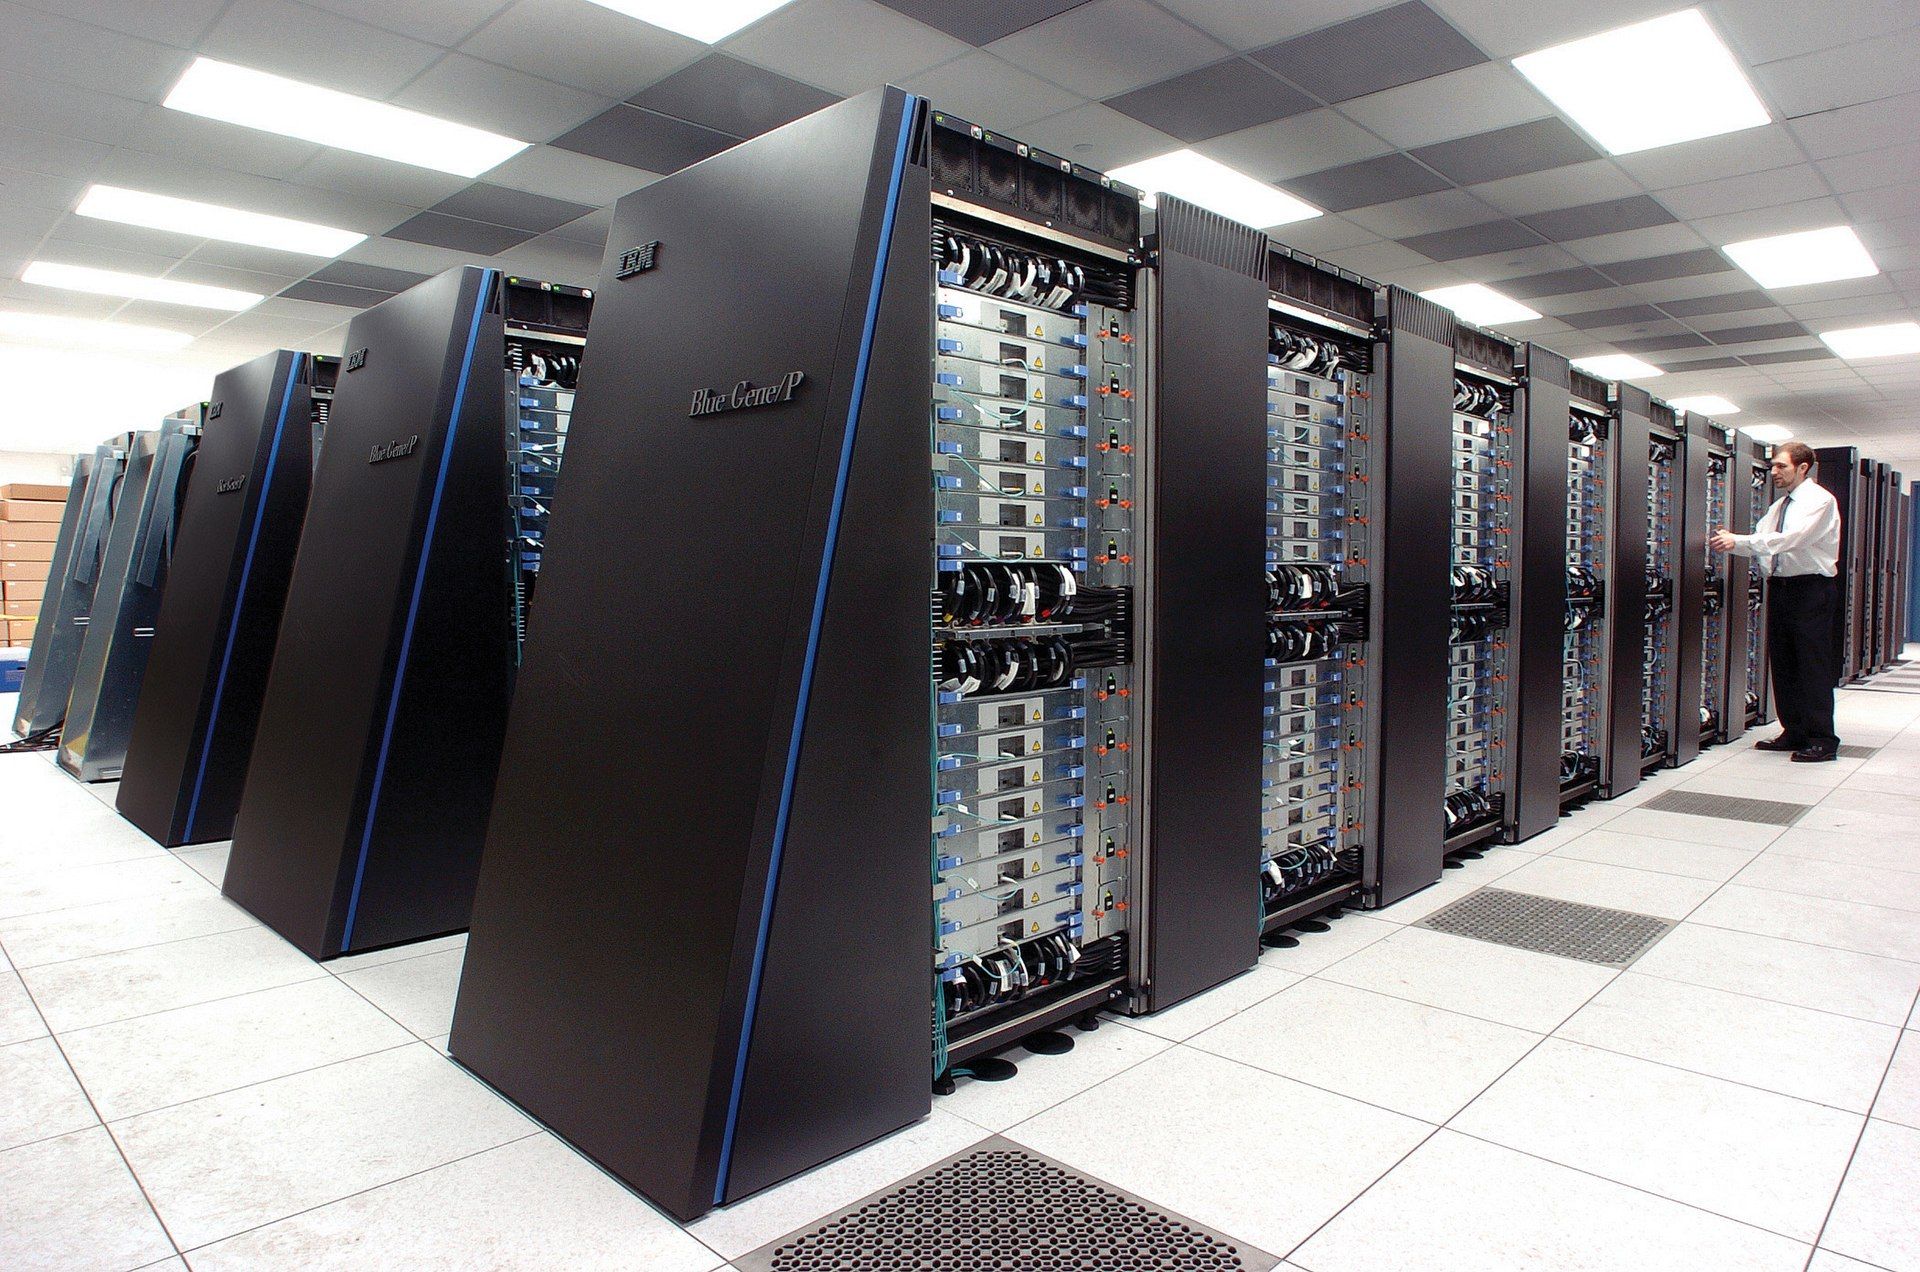
\includegraphics[width=\linewidth]{img/IBM_Blue_Gene_P_supercomputer.jpg}
    \end{column}
    \end{columns}
  \end{block}
  \begin{block}{Exercise 4 p. 3 in the notes}
    \begin{columns}
      \begin{column}{0.6\linewidth}
   Estimate the time it would take you to try all of the possible combinations of the clothes (including accessories!) you choose between each morning. 
      \end{column}
      \begin{column}{0.3\linewidth}
      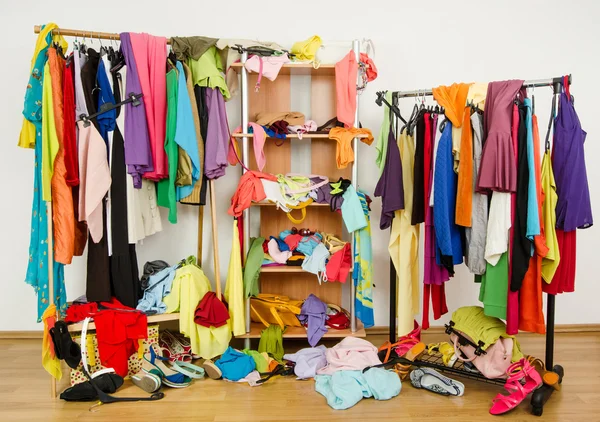
\includegraphics[width=\linewidth]{img/wardrobe.png}
      \end{column}
    \end{columns}
  \end{block}
\end{frame}
\begin{frame}
  \frametitle{Qubits}
  \begin{columns}
    \begin{column}{0.4\linewidth}
      \begin{itemize}
      \item<+-> Qubits are \emph{quantum systems}
      \item<2-> Like Bohr's atomic model
      \item<3-> Qubits are ``simple''. \emph{Only 2 states}
      \item<4-> You know \emph{real simple} like NV Centers...
      \end{itemize}
    \end{column}
    \begin{column}{0.5\linewidth}
      \centering

      \includegraphics<2-3>[width=6cm]{img/bohrmodel.png}

      \includegraphics<4->[width=3cm]{img/nvcenter.png}

      \includegraphics<4->[width=3cm]{img/nvtransitions.png}
    \end{column}
  \end{columns}
\end{frame}

\begin{frame}
  \frametitle{Bits and Qubits}
  \begin{columns}
    \begin{column}{0.5\linewidth}
      \begin{block}{Bits}
        \begin{itemize}
        \item Denoted 0 and 1
        \item If a bit is in state 0 we are sure to measure 0
        \item If a bit is in state 1 we are sure to measure 1
        \item Can \emph{only} be in either state 0 or 1
        \end{itemize}
      \end{block}
    \end{column}
    \begin{column}{0.5\linewidth}
      \begin{block}{Qubits}
        \begin{itemize}
        \item Denoted $\ket{0}$ and $\ket{1}$
        \item If a bit is in state $\ket{0}$ we are sure to measure 0
        \item If a bit is in state $\ket{1}$ we are sure to measure 1
        \item Can be in either state $\ket{0}$, $\ket{1}$ \textbf{or in a superposition of them.}
        \end{itemize}
      \end{block}
    \end{column}
  \end{columns}
  
  \begin{block}<2>{Funny notation}
    A quantum system i described by a state which we denote $\ket{\dots}$.

    It is called a \emph{ket}.
  \end{block}
\end{frame}

  \begin{frame}
    \frametitle{Lingual oddities}
    \begin{columns}
      \begin{column}{0.5\linewidth}
        \begin{itemize}
        \item<1-> Together with a ket, $\ket{\dots}$, there is a 
        \item<2-> \emph{bra}, $\bra{...}$
        \item<3-> Combining them we get a \emph{bra(c)ket}
        \item<4-> or bra(c)ket, $\braket{\dots | \dots}$, like in \emph{parenthesis}
        \end{itemize}
      \end{column}
      \begin{column}{0.4\linewidth}
        \centering
        \includegraphics<2>[width=4cm]{img/bra.jpg}
        \includegraphics<3>[width=4cm]{img/braces.png}
        \includegraphics<4->[width=1cm]{img/brackets.png}
      \end{column}
    \end{columns}
  \end{frame}

\begin{frame}
\section{Superposition}
\centering
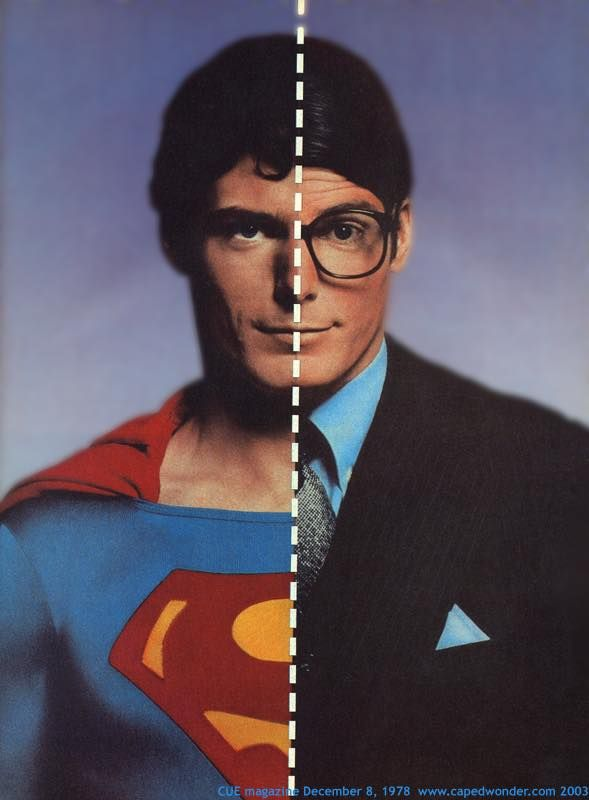
\includegraphics[width=5cm]{img/superman.jpg}
\end{frame}

\begin{frame}
  \frametitle{Single Qubit Superposition}
  \begin{columns}
    \begin{column}{0.49\linewidth}
      A single qubit can be in either:
      \begin{itemize}
      \item<1-|alert@2> state $\ket{0}$
      \item<1-|alert@3> state $\ket{1}$
      \item<4-|alert@4> or in a \textbf{superposition} $\ket{\psi}=\alpha \ket{0}+\beta \ket{1}$
      \end{itemize}
    \end{column}
    \begin{column}{0.5\linewidth}

      \includegraphics<2>[width=\linewidth]{img/clark-kent.png}

      \includegraphics<3>[width=\linewidth]{img/superman.png}

      \includegraphics<4>[width=\linewidth]{img/superman-superposition.png}
    \end{column}
  \end{columns}
\end{frame}

\begin{frame}
  \frametitle{Single Qubit Superposition}
  \begin{columns}
    \begin{column}{0.49\linewidth}
      Or with a coin analogy
      \begin{itemize}
      \item<1-|alert@2> state $\ket{0}$
      \item<1-|alert@3> state $\ket{1}$
      \item<1-|alert@4> or in a \textbf{superposition} $\ket{\psi}=\alpha \ket{0}+\beta \ket{1}$
      \end{itemize}
    \end{column}
    \begin{column}{0.5\linewidth}

      \includegraphics<2>[width=\linewidth]{img/euro-0.jpg}

      \includegraphics<3>[width=\linewidth]{img/euro-1.jpg}

      \includegraphics<4>[width=\linewidth]{img/euro-spinning.png}
    \end{column}
  \end{columns}
\end{frame}

\begin{frame}
  \frametitle{Superposition and normalisation}
  \begin{block}{Definition: Superposition}
    $\ket{\psi}=\alpha \ket{0}+\beta \ket{1}$

    $\alpha$ and $\beta$ can be choosen arbitrarily as long it is \textbf{normalised}.
  \end{block}
  
  \begin{block}{Definition: Normalisation}
    The qubit state $\ket{\psi} = \alpha \ket{0} + \beta \ket{1}$ is normalised if $\alpha^2+\beta^2=1$. 
  \end{block}

  \onslide<2> Read through the example and do exercise 5 and 6 on page 4 in the notes.
\end{frame}

\begin{frame}
  \frametitle{A unit vector}
  \begin{columns}
    \begin{column}{0.5\linewidth}
      \begin{itemize}
      \item $\ket{0} =
        \begin{pmatrix}
          1 \\0 
        \end{pmatrix}
        $ Unit vector along x-axis.
      \item $\ket{1} =
        \begin{pmatrix}
         0 \\ 1 
        \end{pmatrix}$ Unit vector along y-axis.
      \item $\ket{\psi}=\alpha \ket{0}+\beta \ket{1}$ Unit vector pointing from (0,0) to $(\alpha , \beta)$ on the unit circle.
      \end{itemize}
    \end{column}
    \begin{column}{0.49\linewidth}
      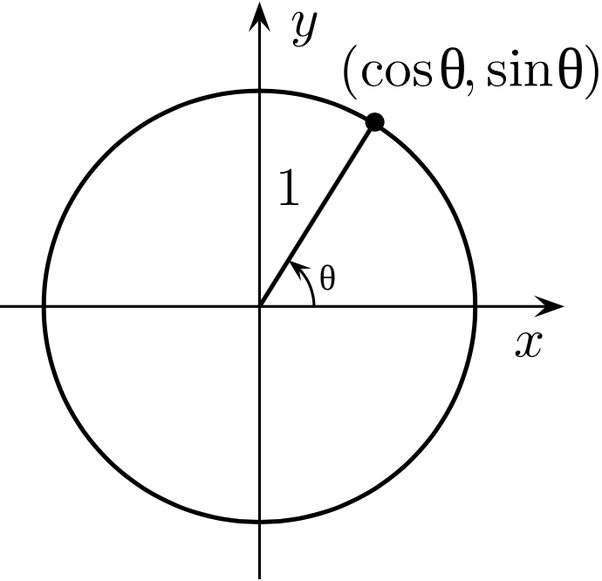
\includegraphics[width=\linewidth]{img/unit-circle.jpg}
    \end{column}
  \end{columns}
  \onslide<2> Do exercise 7 on page 4 in the notes.
\end{frame}
\begin{frame}
  \section{Measurement and Probability}

  \centering
  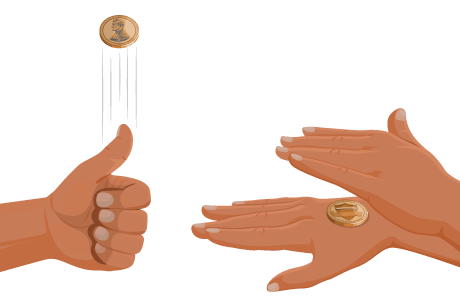
\includegraphics[width=6cm]{img/coin-flip.png}
\end{frame}
\begin{frame}
  \frametitle{Measuring on $\ket{\psi}=\ket{0}$}
  \begin{columns}
    \begin{column}{0.4\linewidth}
      \begin{itemize}
      \item<1-|alert@1> If the qubit is in the state $\ket{\psi}=\ket{0}$
      \item<2-|alert@2> and the quantum computer performs a measurement
      \item<3-|alert@3> we get 0 with 100\% probability.
      \end{itemize}
    \end{column}
    \begin{column}{0.5\linewidth}
      \includegraphics<1>[width=\linewidth]{img/euro-0.jpg}
      \includegraphics<2>[width=\linewidth]{img/coin-measure.png}
      \includegraphics<3>[width=\linewidth]{img/euro-0.jpg}
    \end{column}
  \end{columns}
\end{frame}

\begin{frame}
  \frametitle{Measuring on $\ket{\psi}=\ket{1}$}
  \begin{columns}
    \begin{column}{0.4\linewidth}
      \begin{itemize}
      \item<1-|alert@1> If the qubit is in the state $\ket{\psi}=\ket{1}$
      \item<2-|alert@2> and the quantum computer performs a measurement
      \item<3-|alert@3> we get 1 with 100\% probability.
      \end{itemize}
    \end{column}
    \begin{column}{0.5\linewidth}
      \includegraphics<1>[width=\linewidth]{img/euro-1.jpg}
      \includegraphics<2>[width=\linewidth]{img/coin-measure.png}
      \includegraphics<3>[width=\linewidth]{img/euro-1.jpg}
    \end{column}
  \end{columns}
\end{frame}

\begin{frame}
  \frametitle{Measuring $\ket{\psi}=\alpha \ket{0}+\beta \ket{1}$}
  \begin{columns}
    \begin{column}{0.4\linewidth}
      \begin{itemize}
      \item<1-|alert@1> If the qubit now is in the state $\ket{\psi}=\alpha \ket{0}+\beta \ket{1}$
      \item<2-|alert@2> and the quantum computer performs a measurement.
      \item<3-|alert@3> we get \textbf{either} 0 or 1 and \textbf{never} something in between.
      \item<4-|alert@4> We cannot predict the outcome. Only calculate the probabilities!
      \item<5-|alert@5> We have to abandon \textbf{determinism}.
      \end{itemize}
    \end{column}
    \begin{column}{0.5\linewidth}
      \centering

      \includegraphics<1>[width=\linewidth]{img/euro-spinning.png}

      \includegraphics<2>[width=\linewidth]{img/coin-measure.png}

      \includegraphics<3->[width=3cm]{img/euro-0.jpg}

      \onslide<3-> \Huge or \\

      \includegraphics<3->[width=3cm]{img/euro-1.jpg}
    \end{column}
  \end{columns}
\end{frame}

\begin{frame}
  \frametitle{Probabilities}
  \begin{block}{Definition: Probability}
    If  our qubit is in the state $|\psi\rangle$ then the probability of measuring 0 is given by $P_0 = (\langle0|\psi\rangle)^2$ and the probability of measuring 1 is given by $P_1 = (\langle1|\psi\rangle)^2$.
  \end{block}
  \begin{block}{Rules}
    \begin{equation*}\label{regneregler}
    \braket{0|0}=\braket{1|1}=1 \quad {\rm and} \quad 
        \braket{1}=\braket{1|0}=0
    \end{equation*}
  \end{block}
  \onslide<2>  If you are into vectors, our rules above correspond to taking the dot product of two vectors. The rules $\braket{0|0}=\braket{1|1}=1$ mean that the vectors $\ket{0}$ and $\ket{1}$ both have length 1, and the rules $\braket{0|1}=\braket{1|0}=0$ mean that $\ket{1}$ and $\ket{0}$ are perpendicular.
\end{frame}
\begin{frame}
  \frametitle{Time to work}
  Read through the examples, remarks and do the exercises on page 7 and 8 in the notes.
\end{frame}
\begin{frame}
  \frametitle{The measurement affects the state}
  \begin{columns}
    \begin{column}{0.5\linewidth}
      \begin{itemize}
      \item<1-> A qubit is in a state $\ket{\psi}$
      \item<2-> We do a measurement
      \item<3-> and get 0
        
      \item<4-> We do the same all over again
      \item<5-> A qubit is in a state $\ket{\psi}$
      \item<6-> We do a measurement
      \item<7-> and get 1
      \item<8-|alert@8> What can we say about the state $\ket{\psi}$?
      \item<9-|alert@9> Only that the probabilities $P_0$ and $P_1$ are non zero!
      \end{itemize}
    \end{column}
    \begin{column}{0.5\linewidth}
            \includegraphics<1>[width=\linewidth]{img/euro-spinning.png}
            \includegraphics<2>[width=\linewidth]{img/coin-measure.png}
            \includegraphics<3-4>[width=\linewidth]{img/euro-0.jpg}
            \includegraphics<5>[width=\linewidth]{img/euro-spinning.png}
            \includegraphics<6>[width=\linewidth]{img/coin-measure.png}
            \includegraphics<7->[width=\linewidth]{img/euro-1.jpg}
    \end{column}
  \end{columns}
\end{frame}
\begin{frame}
  \frametitle{Collapse of the state}
  \begin{columns}
    \begin{column}{0.5\linewidth}
      \begin{itemize}
      \item<1-> A qubit is in a state $\ket{\psi}$
      \item<2-> We do a measurement
      \item<3-> and get 0
      \item<4-> We do a measurement again
      \item<5-> and get 0
      \item<6-> and again
      \item<7-> and again
      \item<8-|alert@8> The initial state is collapsed.
      \end{itemize}
    \end{column}
    \begin{column}{0.5\linewidth}
            \includegraphics<1>[width=\linewidth]{img/euro-spinning.png}
            \includegraphics<2>[width=\linewidth]{img/coin-measure.png}
            \includegraphics<3>[width=\linewidth]{img/euro-0.jpg}
            \includegraphics<4>[width=\linewidth]{img/coin-measure.png}
            \includegraphics<5->[width=\linewidth]{img/euro-0.jpg}
    \end{column}
  \end{columns}
      \begin{block}{Definition}<9>
        \footnotesize
        If we measure and the result is 0, then the state of the qubit immediately after the measurement is the state $\ket{0}$. Likewise, if the measurement result is 1, then the state of the qubits immediately after the measurement is the state $\ket{1}$.
      \end{block}
\end{frame}

  \begin{frame}
    \frametitle{Time for some exercise}
    Do exercise 10 on page 8 in the notes.

    \begin{block}{Exercise 10}
      Show that the state $\frac{1}{5}(3\ket{0}+4\ket{1})$ is normalised and determine the probability, $P_1$, of measuring 1 if the qubit is initially in the state $\ket{\psi}=\frac{1}{5}(3\ket{0}+4\ket{1})$.
    \end{block}
  \end{frame}

\begin{frame}
  \section{Operators and Diagrams}
\end{frame}

\begin{frame}
  \frametitle{Single Qubit operators}
  We want to do something with the qubits! We do that with \textbf{operators}.
  \begin{block}{Definition: Operator}
    An operator acts on a state and returns a state.
  \end{block}
\end{frame}

\begin{frame}
  \frametitle{Doing nothing}
  \centerline{\Qcircuit @C=2em @R=1.5em {\lstick{\ket{0}}   &    \qw &    \rstick{\ket{0}} \qw}}
  \vfill
  \begin{itemize}
  \item A single qubit is drawn as a horizontal line. 
  \item Each end indicate the state of the qubit.
  \item Read from left to right.
  \end{itemize}
  \vfill
\end{frame}
  
\begin{frame}
  \frametitle{The Z operator}
  \begin{block}{Definition: The operator Z}
    $Z= \ket{0}\bra{0}-\ket{1}\bra{1}$
  \end{block}
    \centerline{
\Qcircuit @C=2em @R=1.5em {
   \lstick{\ket{0}}   &   \gate{Z}   &    \rstick{\ket{0}} \qw \\
   \lstick{\ket{1}}   &   \gate{Z}   &    \rstick{-\ket{1}} \qw \\
}
}
\begin{itemize}
\item<2-> An operator acts on a state from the \emph{left}.
\item<3->  i.e. $Z \ket{\psi} = \left(\ket{0}\bra{0}-\ket{1}\bra{1}\right) \ket{\psi}$
  
\item<4-|alert@4> What does $Z$ do?
\end{itemize}
\begin{block}{Exercise 15 in the notes.}<4->
  Use the definition of $Z$, i.e. that $Z=|0\rangle\langle0|-|1\rangle\langle1|$, and let it act on $\ket{0}$ and $\ket{1}$. Show that the result is the same as depicted on the figure.
\end{block}
\end{frame}
\begin{frame}
  \frametitle{The X operator}
  \begin{block}{Definition: The operator X}
    $X = \ket{1}\bra{0}+\ket{0}\bra{1}$
  \end{block}
\centerline{
\Qcircuit @C=2em @R=1.5em {
   \lstick{\ket{0}}   &   \gate{X}   &    \rstick{\ket{1}} \qw \\
   \lstick{\ket{1}}   &   \gate{X}   &    \rstick{\ket{0}} \qw \\
}
}
\onslide<2-> What does the X operator do?
\begin{block}{Exercise 16 in the notes.}<2->
  Show what happen when $X$ acts on the state $\frac{1}{\sqrt{2}}(|0\rangle+|1\rangle)$. If you have studied Appendix 2, then note that you have just shown that $\frac{1}{\sqrt{2}}(|0\rangle+|1\rangle)$ is an eigenstate of $X$ with eigenvalue 1!
\end{block}
\end{frame}

\begin{frame}
  \frametitle{The Hadamard operator, $H$}
  \begin{block}{Definition: The operator $H$}
    $H = \frac{1}{\sqrt{2}}\left( \ket{0}\bra{0}+ \ket{0}\bra{1} +\ket{1}\bra{0}-\ket{1}\bra{1} \right)$
  \end{block}	\centerline{
	\Qcircuit @C=1em @R=.7em {
   \lstick{\ket{0}}   & \qw & \gate{H} & \qw & \qw & \rstick{\frac{1}{\sqrt{2}}(\ket{0}+\ket{1})}  \\
   \lstick{\ket{1}}   & \qw & \gate{H} & \qw & \qw & \rstick{\frac{1}{\sqrt{2}}(\ket{0}-\ket{1})}  
}
}
\begin{itemize}
\item<2-|alert@2> Work through the exercises 17, 18, 19 in the notes. Consult the surrounding examples if in doubt or if you need a hint.
\end{itemize}
\end{frame}

\begin{frame}
  \frametitle{Diagrams with measurements}
  \centerline{
\scalebox{1.0}{
\Qcircuit @C=1.0em @R=0.2em @!R { \\
	 	\nghost{{q} :  } & \lstick{{q} : \  \ket{0}} & \gate{\mathrm{X}} % \barrier[0em]{0} 
		& \qw & \meter & \qw & \qw\\
	 	\nghost{\mathrm{{c} :  }} & \lstick{\mathrm{{c} : \ \ \ \ \ \, }} &% \lstick{/_{_{1}}} 
		\cw & \cw & \dstick{_{_{\hspace{0.0em}0}}} \cw \ar @{<=} [-1,0] & \cw & \cw\\
 }}}
\begin{enumerate}
\item<2-> q for \textbf{q}ubit and c for \textbf{c}lassical bit.
\item<3-> qubit starts in state $\ket{0}$
\item<4-> Operator $X$ acts on the state.
\item<5-> The new state is measured (acted on by the measuring operator)
\item<6-> The outcome of the measurement is stored in classical bit number 0 (counting from 0 instead of 1).
\item<7-> The diagram before the measurement translates to the following calculation: $$X \ket{0} = \left(\ket{1}\bra{0} + \ket{0}\bra{1}  \right)\ket{0}$$
\item<8-|alert@8> Predict the outcome of the measurement.
\end{enumerate}
\end{frame}

\begin{frame}
  \frametitle{Example and exercise}
  Read through the example concerning the Hadamard operator on page 17 and 18 in the notes.
  Then do exercise 21 on page 18 in the notes.

  \begin{block}{Exercise 21}
   \centerline{
\scalebox{1.0}{
\Qcircuit @C=1.0em @R=0.2em @!R { \\
	 	\nghost{{q} :  } & \lstick{{q} : \  \ket{0}  } & \gate{\mathrm{H}} & \gate{\mathrm{Z}}  %\barrier[0em]{0}
		 & \qw & \meter & \qw & \qw\\
	 	\nghost{\mathrm{{c} :  }} & \lstick{\mathrm{{c} :  \ \ \ \ \ \,  }} & % \lstick{/_{_{1}}} 
		\cw & \cw & \cw & \dstick{_{_{\hspace{0.0em}0}}} \cw \ar @{<=} [-1,0] & \cw & \cw\\
\\ }}
} 

Our qubit start out in the state $\ket{0}$. Explain what the state of our qubit is after $H$ and then $Z$ have acted on it, i.e. calculate $ZH\ket{0}$. Then determine what the probability is of measurement giving 0 and 1, respectively.
  \end{block}
\end{frame}
\begin{frame}
  \centering
  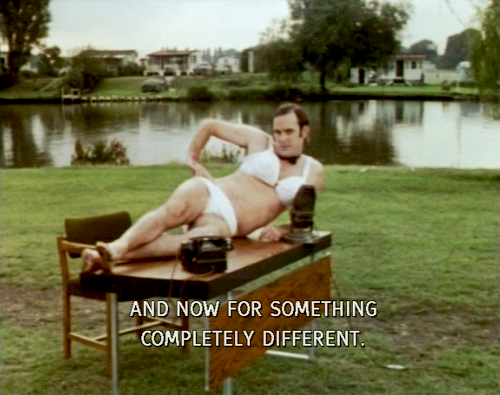
\includegraphics[width=8cm]{img/completely-different.png}
  \uncover<2->{
    \begin{tikzpicture}[overlay, remember picture]
     \draw[red,thick] (-4.1,0.9) -- (-2.3,0.9);
     \node[align=left,anchor=west,red, thick] at (-4.1,0.7) {RELATED.};
    \end{tikzpicture}
      }
\end{frame}
\begin{frame}
  \section{IBM Q}
  \centering
  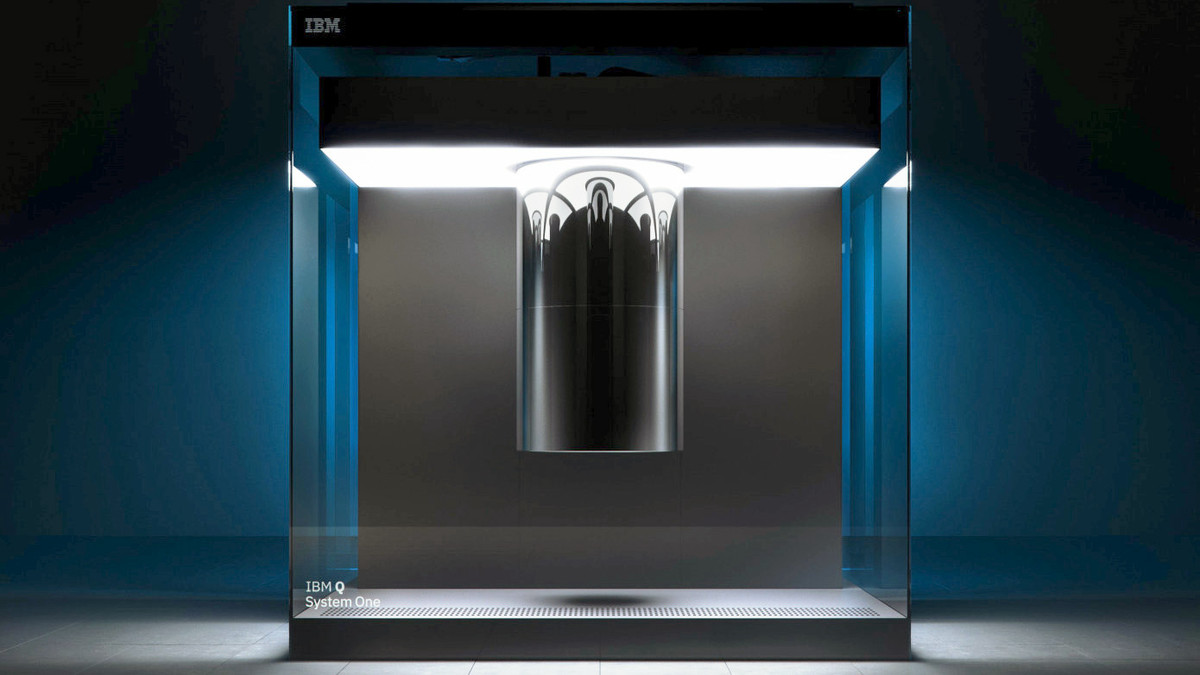
\includegraphics[width=0.7\linewidth]{img/IBMQ.jpg}
\end{frame}

\begin{frame}
  \frametitle{Access IBM Q}
  \begin{itemize}
  \item Visit \href{https://quantum-computing.ibm.com/}{https://quantum-computing.ibm.com/}
  \item Create an IBM account or sign in with one of the other options.
  \item Go to ``Lab''.
  \end{itemize}
  \centering
  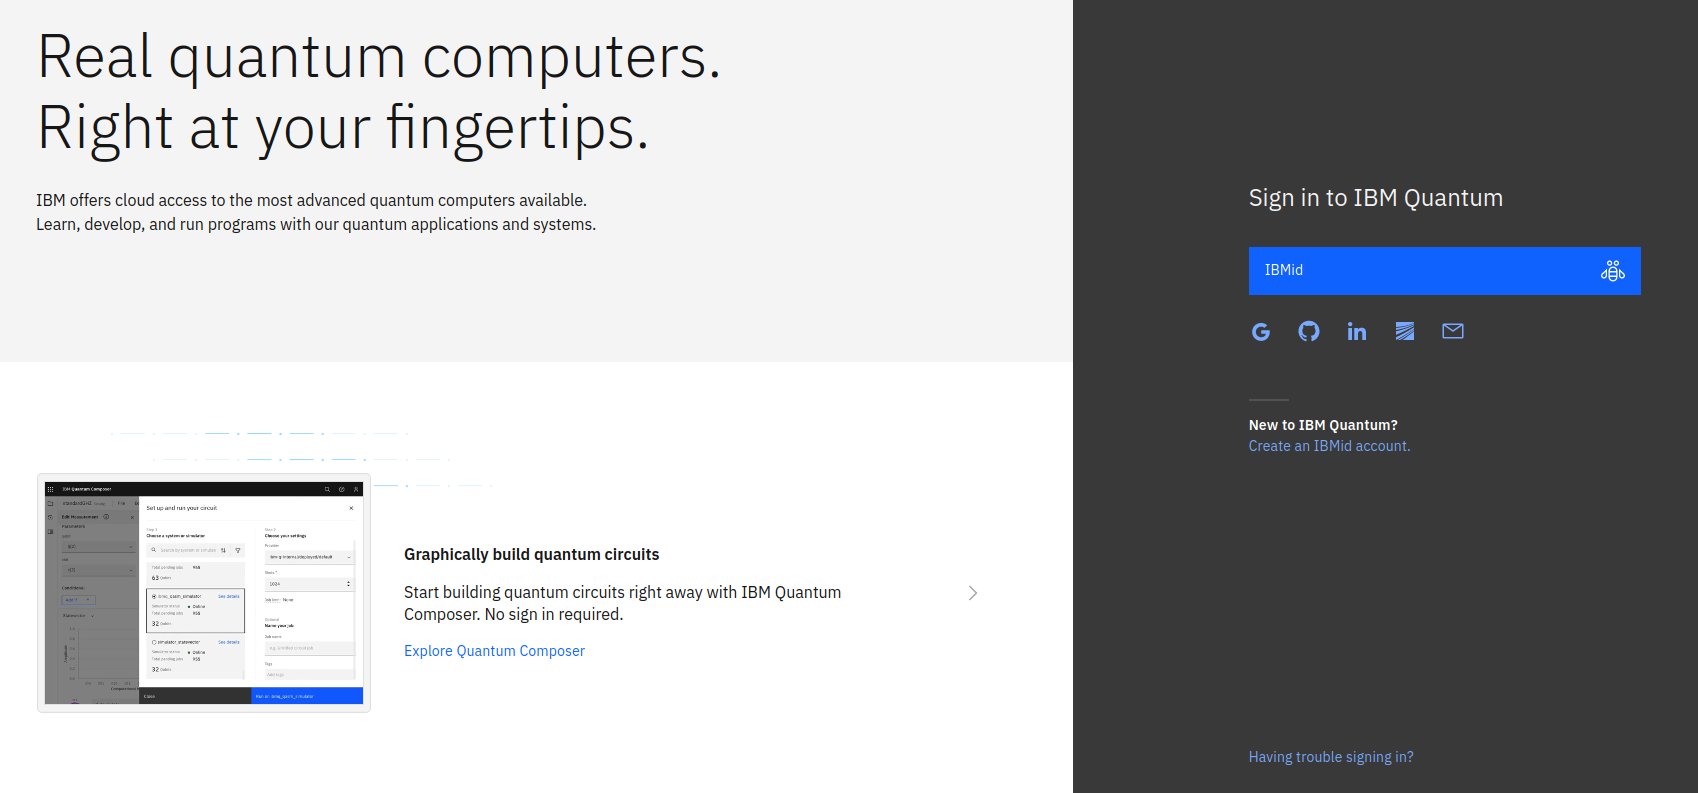
\includegraphics[width=9cm]{img/ibmq-login.png}
\end{frame}

\begin{frame}
  \frametitle{Upload the IBM Q exercises}
  Upload the following exercises to the lab file browser. (You can use drag and drop).
  \begin{itemize}
  \item MeasurementSingleQubit.ipynb
  \item MeasurementTwoQubits.ipynb
  \item MeasurementEntangledQubits.ipynb
  \item GroversAlgorithm.ipynb
  \end{itemize}

  \centering
  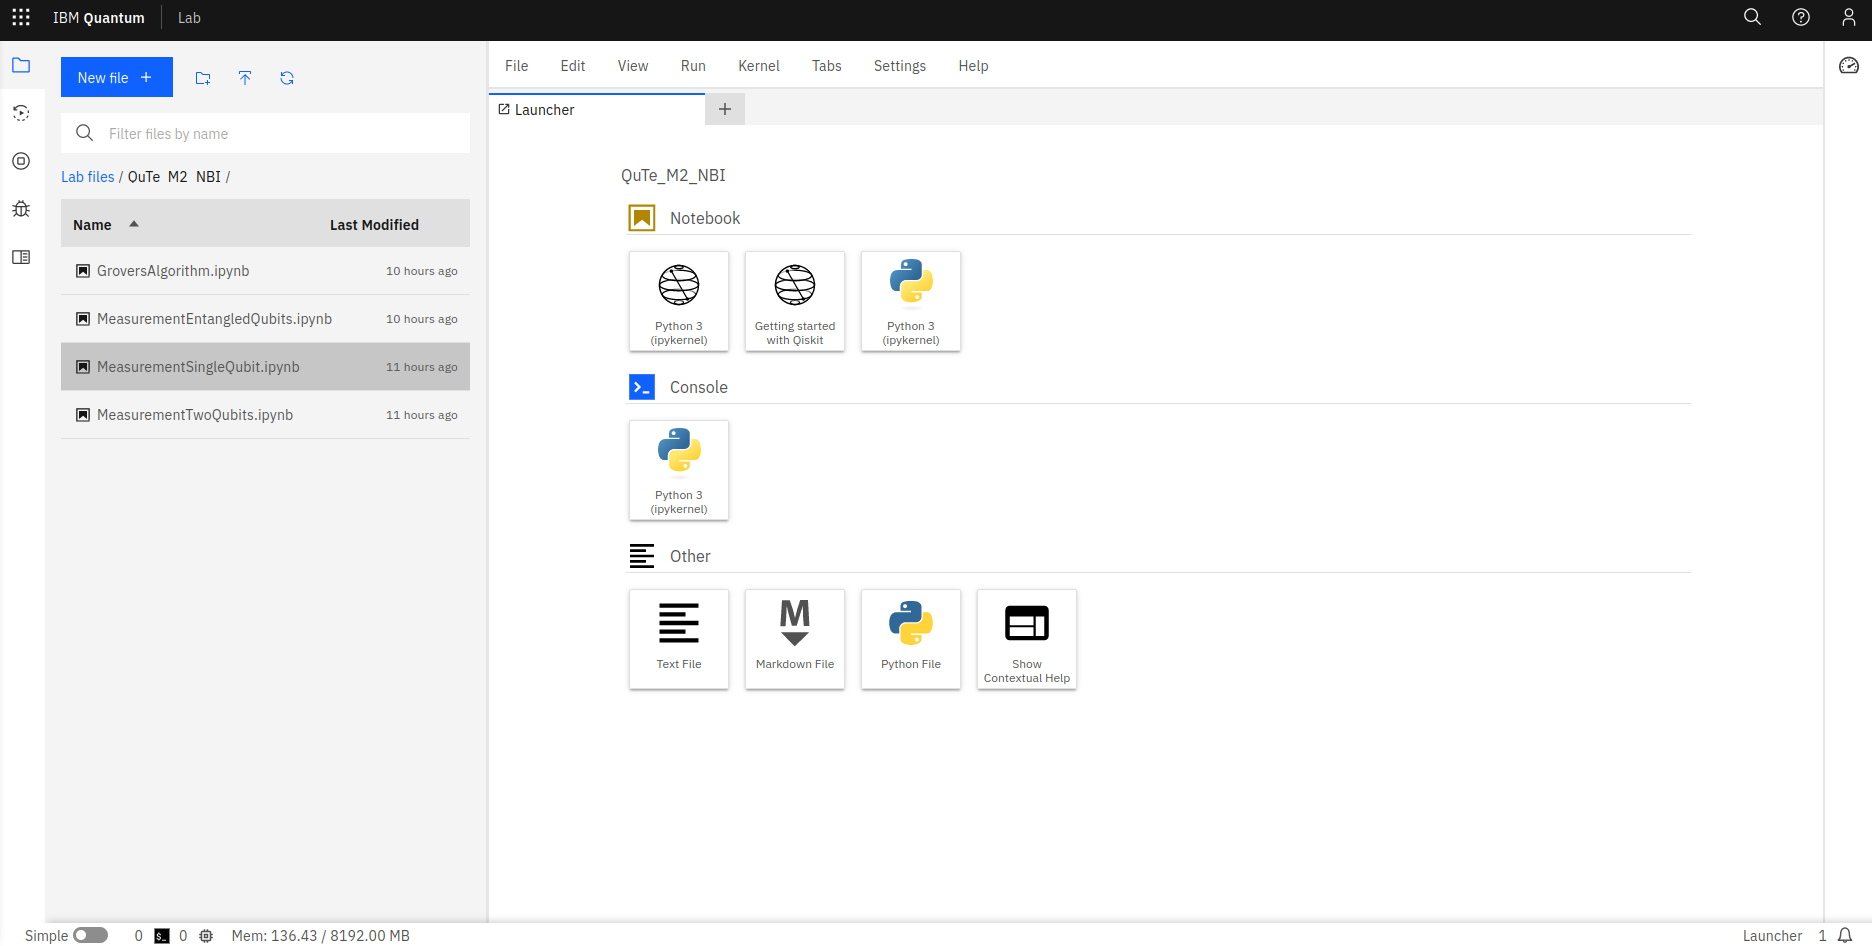
\includegraphics[width=9cm]{img/ibmq-upload.png}
\end{frame}

\begin{frame}
  \frametitle{Single Qubit Measurements}
  Run the \emph{Measurement SingleQubit.ipynb} notebook and follow the instructions. You are now able to perform \textbf{real} work on a real \textbf{quantum computer}! (If you set the variable sym=False)
  \begin{center}
  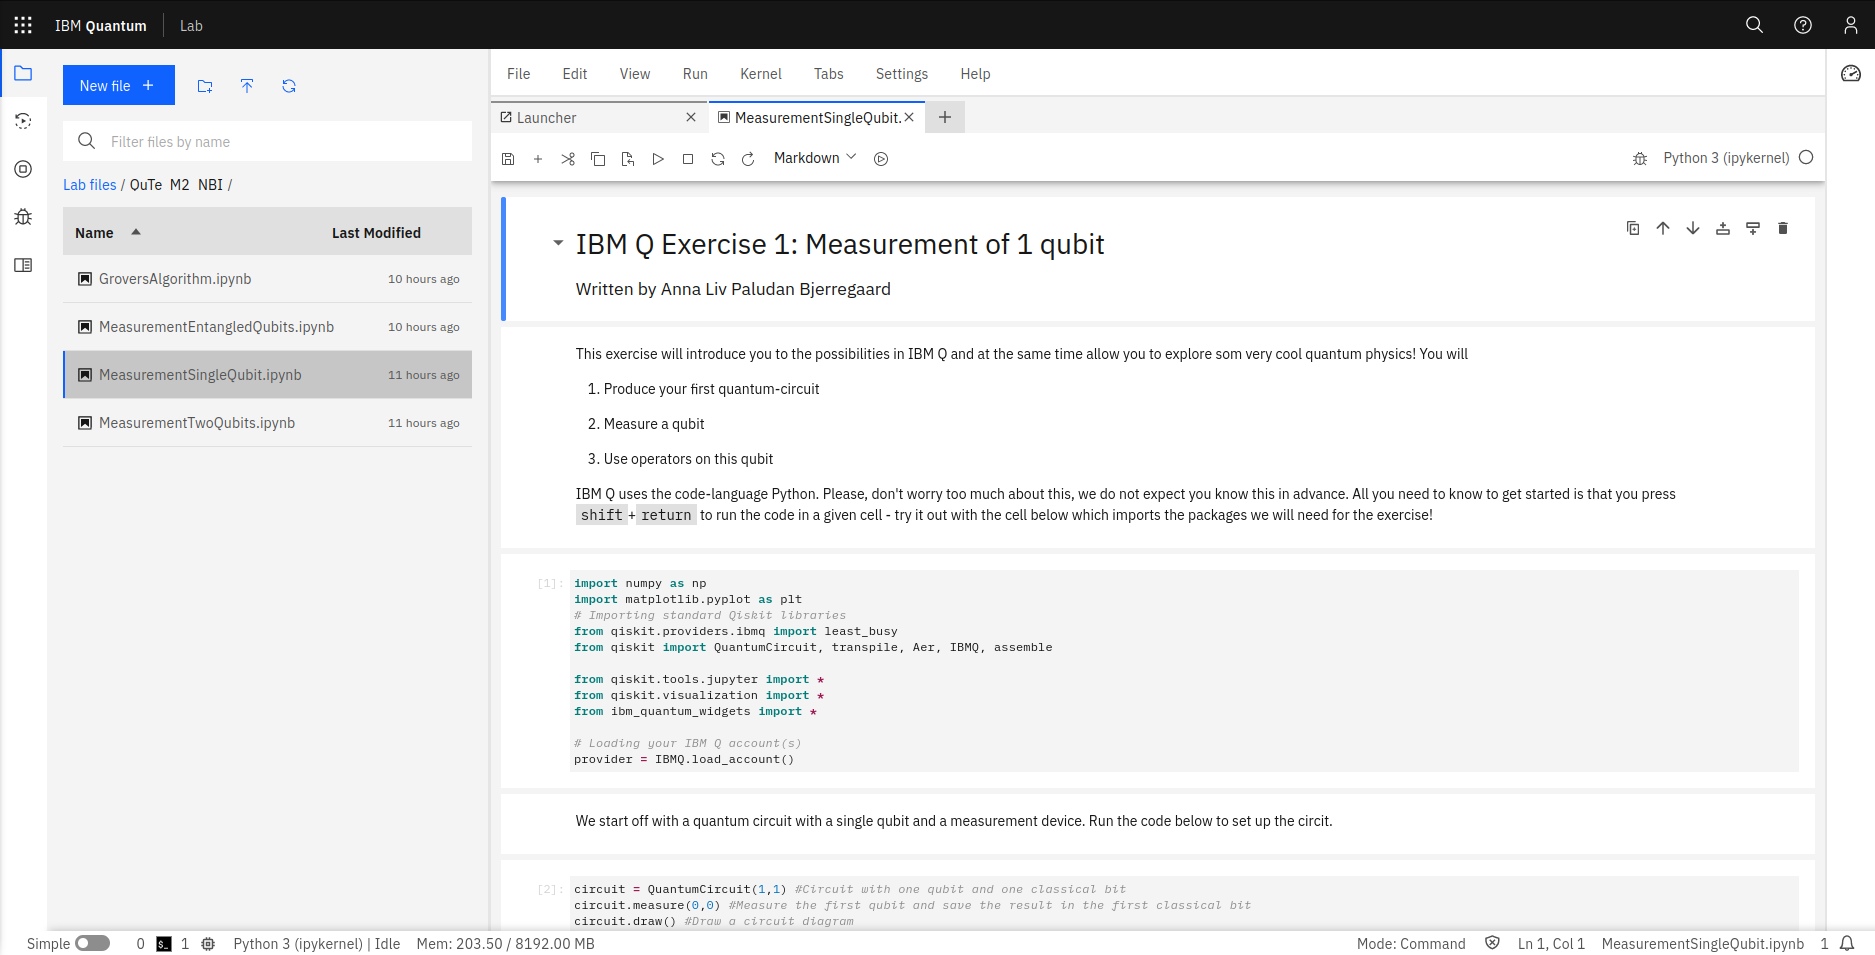
\includegraphics[width=10cm]{img/ibmq-single-qubit.png}
  \end{center}
\end{frame}

\begin{frame}
  \frametitle{Pun intended!}
 Did you get the pun? 
  \begin{center}
  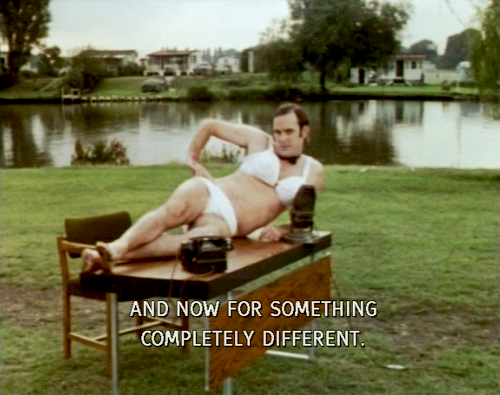
\includegraphics[width=7.5cm]{img/completely-different.png}
    \begin{tikzpicture}[overlay, remember picture]
     \draw[red,thick] (-4.1,0.9) -- (-2.3,0.9);
     \node[align=left,anchor=west,red, thick] at (-4.1,0.7) {RELATED.};
    \end{tikzpicture}
  \end{center}
  \uncover<2->{Monty Python $\to$ IBM Q \emph{is} related $\to$ IBM Q uses \emph{Python} $\to$ Python is named after Monty Python, because programming should be fun!}
\end{frame}

\begin{frame}
  \frametitle{Back to school!}
  \centering
  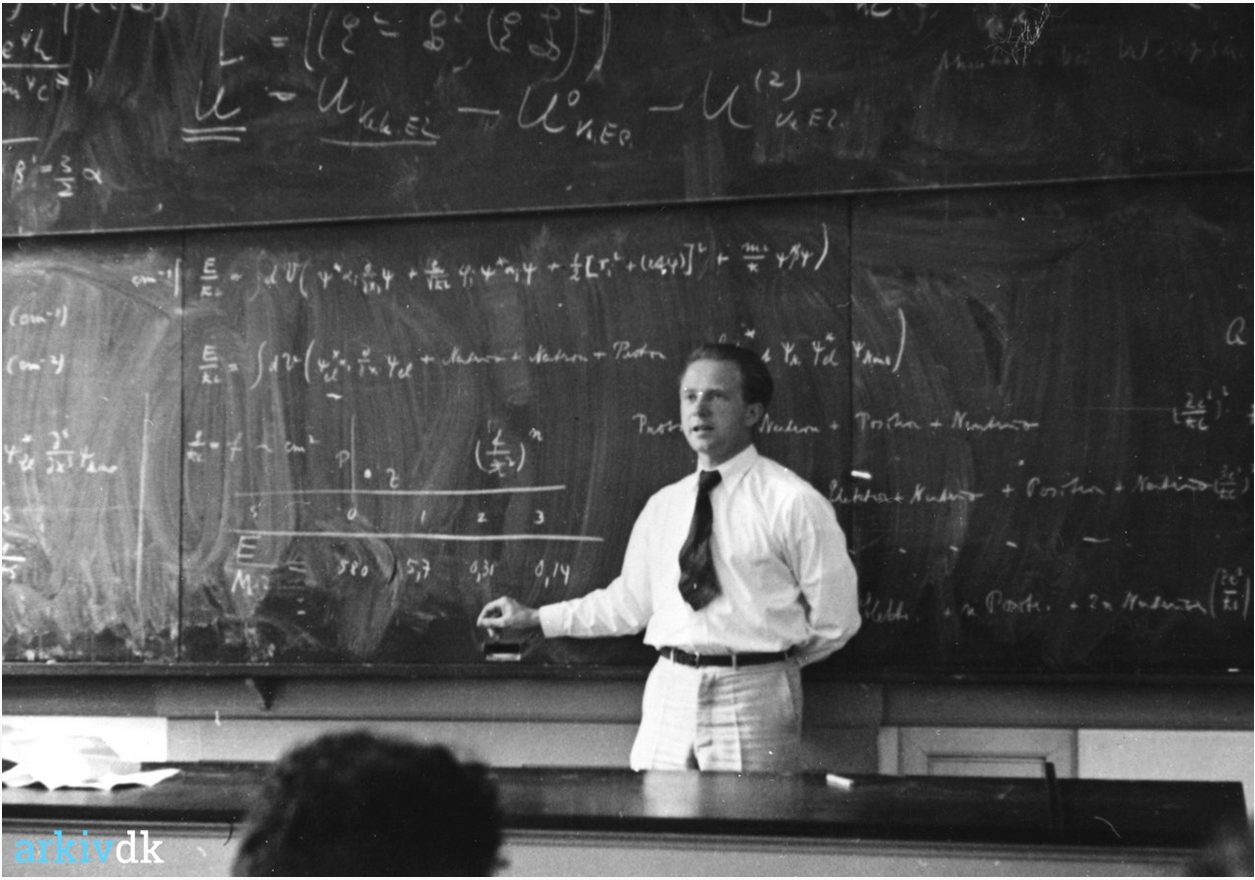
\includegraphics[width=10cm]{img/back-to-school.png}
\end{frame}

\begin{frame}
  \section{Two Qubit Measurements}
\end{frame}
\begin{frame}
  \section{Entanglement}
  \centering
  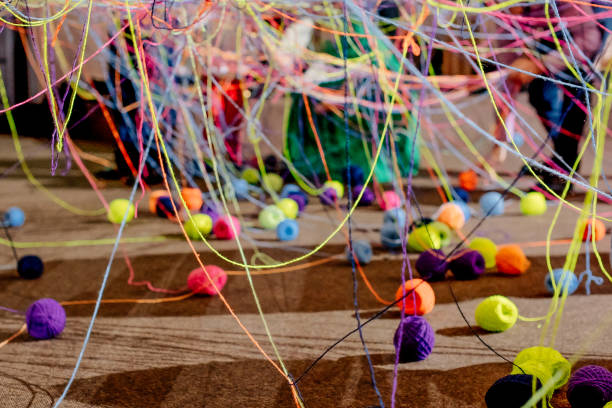
\includegraphics[width=0.7\linewidth]{img/tangled-yarn.jpg}
\end{frame}

\begin{frame}
  \frametitle{Back to IBM Q}
  \centering
  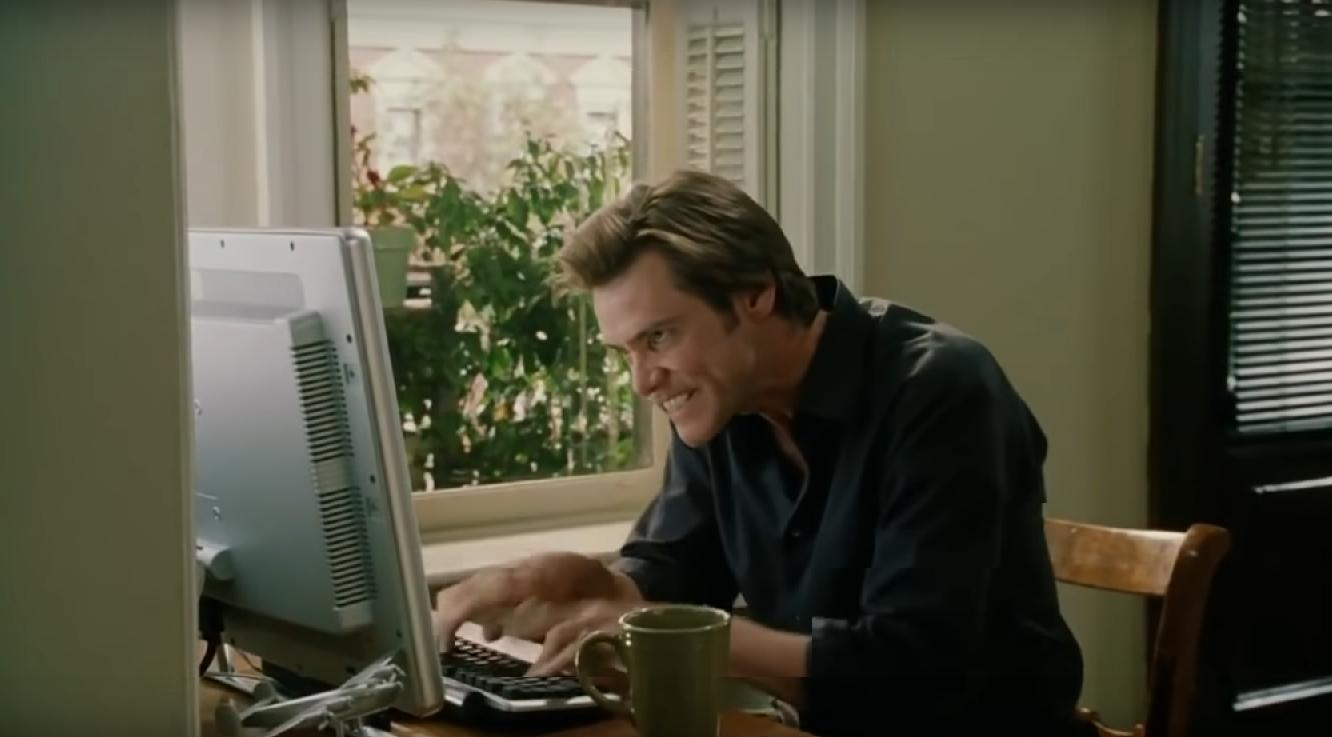
\includegraphics[width=10cm]{img/typing.jpg}
\end{frame}

\end{document}